        \subsection{number formats} 

	\begin{frame}\frametitle{sampling and quantization}\framesubtitle{quantization: word length and SNR}
			\begin{table}
			\centering
				\begin{footnotesize}
					\begin{tabular}{lccc}
					\hline
						\textbf{w} & \textbf{$\Delta$} & \textbf{Max.\ Amp} & \textbf{theo.\ SNR} \\
					\hline
						8 (Int)	&	$\pm1$ & $0\ldots255$ & $\approx$\unit[48]{dB}\\
						16 (Int)	&	$\pm1$ & $-32768\ldots32767$ & $\approx$\unit[96]{dB}\\
						20 (Int)	&	$\pm1$ & $-524288\ldots524287$ & $\approx$\unit[120]{dB}\\
						24 (Int)	&	$\pm1$ & $-16777216\ldots16777215$ & $\approx$\unit[144]{dB}\\
					\hline
						32 (Float)	&	$\pm1.175\cdot10^{-38}$ & $\pm3.403\cdot10^{1038}$ & \unit[1529]{dB}\\
						64 (Float)	&	$\pm2.225\cdot10^{-308}$ & $\pm1.798\cdot10^{10308}$ & \unit[12318]{dB}\\
					\hline
					\end{tabular}  
				\end{footnotesize}
			\end{table}
			\pause
			value range
			\begin{itemize}
				\item	\textbf{unnormalized}: $-2^{w-1}\ldots 2^{w-1}-1$
				\item	\textbf{normalized} (word length independent): $-1\ldots 1$
			\end{itemize}
	\end{frame}	

	\begin{frame}\frametitle{sampling and quantization}\framesubtitle{number representation 1/2}
	    \begin{figure}
			\centering
				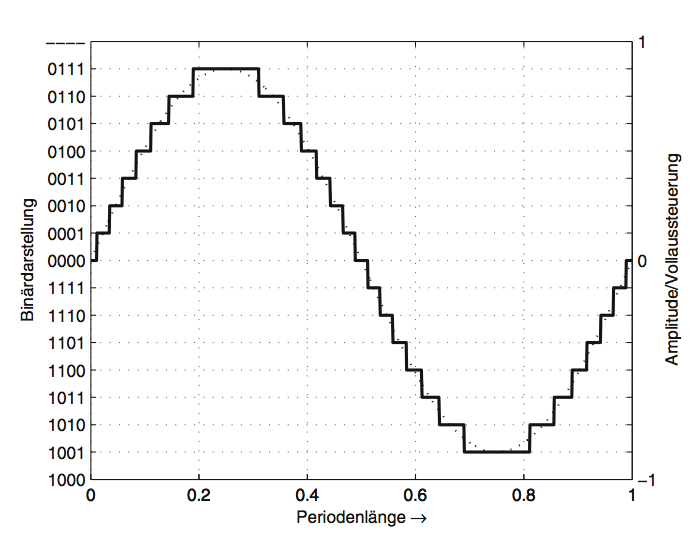
\includegraphics[scale=0.6]{Graph/2complement}
		\end{figure}
		\begin{itemize}
			\item	Least Significant Bit (LSB): $b_0$
			\item	Most Significant Bit (MSB): $b_{w-1}$
		\end{itemize}
	\end{frame}	

	\begin{frame}\frametitle{sampling and quantization}\framesubtitle{number representation 2/2}
		\begin{table}
			\centering
			\begin{footnotesize}
				\begin{tabular}{clc}
				\hline
				\textbf{format} & \textbf{amplitude} & \textbf{range (normalized)}\\
				\hline
				2-Complement & $x_Q = -b_{w-1} + \sum\limits_{i=0}^{w-2}b_{i}2^{-(w-i-1)}$ & $-1\leq x_Q \leq 1-2^{-(w-1)}$\\
				unsigned & $x_Q = \sum\limits_{i=0}^{w-1}b_i2^{-(w-1)}$ & $0\leq x_Q \leq 1-2^{-w}$\\
				\hline
				\end{tabular}
			\end{footnotesize}
		\end{table}
		\begin{itemize}
			\item	$w:$ word length
			\item	$b_i:$ ith Bit
		\end{itemize}
	\end{frame}
	
	\begin{frame}\frametitle{sampling and quantization}\framesubtitle{quantization: clipping \& wrap-around}
	    \begin{figure}
	    	\centering
				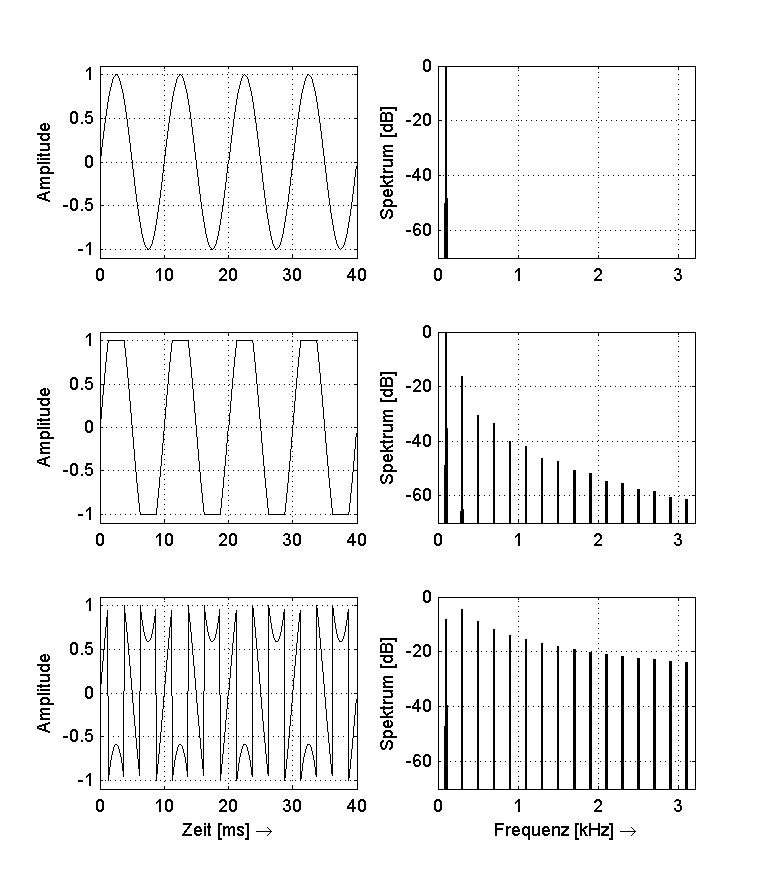
\includegraphics[scale=0.5]{Graph/Lerch14-11}
		\end{figure}
	\end{frame}	
	
	\begin{frame}\frametitle{sampling and quantization}\framesubtitle{fixed point and floating point}
	
		number formats and their most frequent uses
		\begin{itemize}
			\item	\textbf{unsigned format}: small word lengths (4\ldots 8 Bit)
			\pause
			\item	\textbf{2's complement}: file formats with higher word lengths (16\ldots 24 Bit), some DSPs
			\pause
			\item	\only<4>{\textcolor{gtgold}}{\textbf{floating point}}: internal representation for processing
		\end{itemize}
	\end{frame}	
	
	\begin{frame}\frametitle{sampling and quantization}\framesubtitle{floating point 1/2}
		\begin{equation}
		x_Q = M_G \cdot 2^{E_G}
		\end{equation}
		
		\begin{itemize}
			\item	$M_G$: Normalized Mantissa $ 0.5 \leq M_{G} < 1$
			\item	$E_G$: Exponent
		\end{itemize}
		
		\pause
		\textbf{32 Bit IEEE 754 Floating Format}:
		\begin{table}
			\centering
			\begin{footnotesize}
				\begin{tabular}{ccc}
				\hline
				\textbf{Bit 31: Sign} & \textbf{Bits 30-23: Exponent} & \textbf{Bits 22-0: Mantissa}\\
				\hline
				$s$ & $e_{7}$ ... $e_{0}$ & $m_{22}$ ... $m_{0}$\\
				\hline
				\end{tabular}
			\end{footnotesize}
		\end{table}
		\pause
		\textit{Exceptions}
		\vspace{-3mm}
		\begin{table}
			\centering
			\begin{footnotesize}
					\begin{tabular}{cccl}
					\hline
					\textbf{Typ} & \textbf{$E_G$} & \textbf{$M_{G}$} & \textbf{Value}\\
					\hline 
					normal & $1\leq E_G \leq 254$ & any & $(-1)^s (0.m)2^{E_G-127}$\\
					\hline
					NAN (not a number)& 255 & $\neq 0$ & undefined\\
					\hline
					Infinity & 255 & $=0$ & $\infty$\\
					\hline
					Zero & 0 & 0 & 0\\
					\hline
					\end{tabular}
			\end{footnotesize}
		\end{table}
	\end{frame}	
	
	\begin{frame}\frametitle{sampling and quantization}\framesubtitle{floating point 2/2}
		\begin{columns}
			\column{5cm}
			\begin{figure}
				\centering
					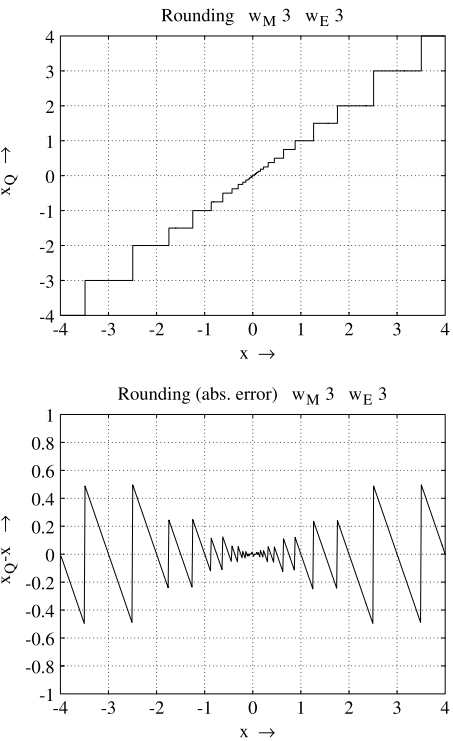
\includegraphics[scale=0.35]{Graph/floatquanterror}
			\end{figure}
			
			\column{4cm}
			\pause
			\begin{itemize}
				\item	\textbf{high exponent}: large quantization error energy
				\item	\textbf{low exponent}: small quantization error energy
			    \pause
                \bigskip
                \item	\textbf{linear quantization} within one exponent
			\end{itemize}
		\end{columns}
	\end{frame}	
